\documentclass[11pt,a4paper]{article}
\usepackage[utf8]{inputenc}
\usepackage[left=2cm,text={17cm, 24cm},top=3cm]{geometry}
\usepackage{times}
\usepackage[english]{babel}
\usepackage[T1]{fontenc}

\author{Alena Tesařová}
\usepackage[ruled,english,linesnumbered,longend,noline]{algorithm2e}
\usepackage{graphics}
\usepackage{float}

\DeclareGraphicsExtensions{.png,.pdf}
\usepackage{hyperref}
\usepackage{cprotect}
\usepackage{graphicx}

\usepackage{pdflscape}
\usepackage{multirow}
\usepackage[binary-units=true]{siunitx}
\usepackage{url}
\usepackage[T1]{fontenc}

\begin{document}

\begin{titlepage}

\begin{center}
\Huge
\textsc{Fakulta informačních technologií\\
Vysoké učení technické v~Brně}\\
\vspace{\stretch{0.382}}
\Huge Nástroje monitorující a generující zprávy jednoduchých distance-vector protokolů
\\
\medskip
{\Large ISA 2018}
\vspace{\stretch{0.618}}
\end{center}


\begin{LARGE}
\noindent

\end{LARGE}
{\Large 
Alena Tesařová (xtesar36)
}
\hfill
{\Large 
\today
}
\end{titlepage}




\section{Abstract}
In internet it is not likely to have one single protocol that is used for the entire network. Rather, network is divided into autonomous systems (AS) where each AS has its own routing technology. Although there are many types of protocol that determines communication between nodes, we can divide them into 2 groups Interior gateway protocol (IGP) and Exterior gateway protocol (EGP). IGP is a routing protocol used in AS and a EGP is used to transfer information among ASs. RIP is designed to work as an IGP in moderate-size AS.  

\section{Routing information protocol}
RIP is a distance-vector routing protocol used in smaller networks, that sends the complete routing table out to all interfaces every 30 seconds. RIP only uses hops to determine the best way to a remote network. However there is a maximum hop count of 15 by default (16 means unreachable). RIP version 1 uses mechanism called classful routing meaning that all devices in the network must use same subnet mask. The reason is that RIPv1 doesn't send updates with subnet mask information. On the other hand RIPv2 provides classful routing and sends subnet mask with the route updates\cite{book}.

\noindent
RIPv2 as a newer protocol should solve problems that appeared in version one. There is a short recapitulation of differences between Ripv1 and RIPv2. 

\subsubsection{Differences between protocols}

\textbf{RIPV1}
\begin{itemize}
\item no authentication
\item no support for discontiguous\footnote{By definition, contiguous means next or together in sequence, \url{https://learningnetwork.cisco.com/thread/30426}} networks
\item classful
\item broadcast based
\item no support for variable long subnet mask(VLSM)
\end{itemize}

\noindent
\textbf{RIPV2}
\begin{itemize}
\item allows MD5 authentication
\item supports discontiguous networks
\item classless
\item uses multicast 244.0.0.9
\item support for VLSM
\end{itemize}

\subsubsection{Controls}
There are more controls on RIP packet that we have to keep in mind while programming RIP.

\noindent
Response must be ignored if:
\begin{itemize}
\item ip address is not from right UDP port
\item source of datagram must be from link local address
\item if the metric is greater than 16, ignore the entry but log the event
\end{itemize}

\subsubsection{Common limitations}
\begin{enumerate}
\item maximum of 15 hops
\item counting to infinity to resolve certain unusual situations (if it was immense it would require either much time or bandwidth)
\item uses fixed metrics (no real time factors as delay, reliability, load)
\end{enumerate}



\subsubsection{Structure of RIP}
\label{sec:ripv4}
RIP protocols are designed to have one header ($\SI{4}{\byte}$) and several entries (each $\SI{20}{\byte}$). RIP header contains information as version of RIP and command (either request or response). In entries we find address family identifier (\texttt{AFI}) describing type of address ($\SI{4}{\byte}$), route tag ($\SI{4}{\byte}$), which differs external rip routes from internal or it can be also a type of authentication. If an address family identifier equals \texttt{0xFFFF}, then according to the authentication type we parse authentication data ($\SI{16}{\byte}$). To see more information about authentication go to section~\ref{sec:auth}. If \texttt{AFI} equals value of \texttt{AF\_INET}, then subnet mask ($\SI{4}{\byte}$), destination IPv4 address ($\SI{4}{\byte}$), next hop\footnote{address of next router along the path to the destination} ($\SI{4}{\byte}$) and the cost to reach that destination (called metric, $\SI{4}{\byte}$) are sent.

\subsubsection{RIP header}
All RIP protocols have same header that contains version, zeros and type of message. There are two types of message: Request and Response.

\begin{itemize}
\item \textbf{Request}
\begin{itemize}
\item used to ask for response containing all or part of a routers routing table  
\item normally is sent as multicast (broadcast for RIPv1) but there can be a situation that we need to send just one response to just one router (possible with RIPng) then packet is sent directly to the router from an UDP port other that the RIPng port
\item if there is one entry in the request, destination prefix is zero, a prefix length is zero, metric of infinity 16, then this is a request to send entire routing table
\end{itemize}

\item \textbf{Response}
A response A message containing all or part of the sender's routing table.  It can be sent in response to a request or it may be a routing update generated by the sender.
There 3 reasons to send a response:
\begin{itemize}
\item response to a query
\item regular update
\item triggered update caused by a route change
\end{itemize}
\end{itemize}

\noindent
To conclude, RIPv2 is an advanced RIPv1 which can be used in small networks or at the edge of larger networks because of its simplicity in usage and configuration.

\subsubsection{Authentication}
\label{sec:auth}
Security is one of the primary concerns of network designers today\cite{auth}. Our main concern in RIP protocols is to ensure that information entered into the routing table is valid or not. An attacker can easily send a malicious packet that will be sent to network and might end up in the routing table due to poor configuration. Because of this, it's necessary to authenticate the routing update process. Either we can authenticate an update with Simple or MD5 authentication (RIPv2). The difference is clear, the simple password is sent through network as a plain text for everybody to see compared to MD5 that sends encrypted data to be decoded by a specific authentication algorithm.
\\ \\
\textbf{MD5 authentication}\\
\noindent
Configuration of MD5 consists of:

\begin{enumerate}
\item defining a key chain with a name that determines the set of keys that can be used on the interface
\item defining the key or keys on the chain (related to number point number one)
\item defining the key string to be used in the key, needs to be same on remote routers, the actual password
\item enabling authentication on the interface and specifying the key chain + type of authentication (MD5)
\end{enumerate}

\noindent
Apart from type number 3, routing update contains:
\begin{enumerate}
\item $\SI{16}{\bit}$ authentication data (not in the same entry as Key Identifier)
\item $\SI{8}{\bit}$ field contains Key Identifier or Key id
\item $\SI{8}{\bit}$ field contains the length of data field
\item $\SI{32}{\bit}$ sequence number that must be non-decreasing for all message with same key ID
\end{enumerate}

\noindent
Verification uses MD5 hash algorithm using a password which routing updates does not carry (that makes is authenticate). Rather, it carries a $\SI{16}{\bit}$ message, generated by the MD5 algorithm on the password.


\subsection{RIPng}
Protocol RIPng is a routing protocol implemented for IPv6 networking. In comparison with RIPv2 there is no authentication, RIPng relies on the IP Authentication Header\cite{ip_header} and the IP Encapsulating Security Payload\cite{payload}\cite{ripng}. Structure is similar to RIPv2 described in \ref{sec:ripv4}, but instead of sending subnet mask, a prefix length is sent. 


\section{Implementation details}
Our main task was to study routing protocols RIP, RIP2 and RIPng. After that, we implemented sniffer RIPv1, RIPv2 and RIPng messages, faker that sends a RIP response message to router and perform a success attack.

\subsection{Sniffer}
There is a an example how to run the program after compilation (after make). Program sniffers all RIP packets and format them on output.\\

\noindent
\texttt{format: ./myripsniffer -i <interface>}\\
\texttt{example: ./myripsniffer -i eth0}

\subsubsection{File structure}
\texttt{sniffer.c} - contains functions to parse and print RIP packets (RIPv1, RIPv2, RIPng)\\
\texttt{headers.h} - contains RIP packets headers\\
\texttt{sniffer\_h.h} - contains headers of functions belonging to RIP sniffer\\
\texttt{myripsniffer.c} - main file that starts capturing packets\\

\noindent
For capturing packets I was using functions from libpcap library. Firstly is important to set an interface, open a handle and apply a filter. Chosen filter was udp port $520$ or udp port $521$ that corresponds to RIPv1, RIPv2 and RIPng protocols. In an immense loop (function \texttt{pcap\_loop}), I was parsing packets and printing all important information (function \texttt{print\_packet}). Thanks to libraries as \texttt{ip.h, udp.h}, I did not have to implement structure of udp and ip protocol. I implemented RIP structures described in \ref{sec:ripv4} in file \texttt{headers.h} and had to distinguish IPv4 packets from IPv6 packets (functions \texttt{ipv6\_process} and \texttt{ipv4\_process}). Due to a fact that we know a routing table entry length and length of RIP packet, we can loop till actual parsing length is equal or greater than rip length. In this loop I parse RIP entry, for IPv4 we must not forget types of authentication (see more in section \ref{sec:auth}).

\subsection{RIP response}
There is a an example how to run the program sending one rip packet after compilation (after make). Program send RIP packet according to information given on input.\\

\noindent
\texttt{format: ./myripresponse -i <interface> -r <IPv6>/[16-128] {-n <IPv6>} {-m [0-16]} \\{-t [0-65535]}} \\
\texttt{example: ./myripresponse -i eth0 -r 2001:db8:0:abcd::/64 }\\

\subsubsection{Structure}
\texttt{myripresponse.c} - main file for rip response, parse and process all arguments\\
\texttt{response.c} - file to create and send rip packet\\
\texttt{response.h} - contains used response structures\\

\noindent
This part of project is shorter than the first one. It is composed of two parts - parsing arguments and sending a RIPng packet. This packet consists of one RIP header and two routing table entries. In header we set response command and version one. First entry contains next hop with metric of value of \texttt{0xFF}\cite{ripng} and the second contains information given on input (route tag, prefix, number of hops, metric). Next hop is set according to input or a default next hop is used (\texttt{::}). This order is specified in RFC 2080.\\

\noindent
While creating a UDP packet, we set a receiver's address to multicast group \texttt{FF02::9}, RIPng port $521$, interface index, hop limit of $255$ (maximum hop limit), \texttt{AFI} and receiver's IPv6 address to any (\texttt{in6addr\_any}).

\section{Testing}
\subsection{Settings}
On my computer I have two virtual machines with FreeBSD (given from school) and Ubuntu that I run on VirtualBox. Both machines are set on internal network with same name of the network to be able to see each other. While testing, I run Wireshark on Ubuntu and compare results with my program. As a result I can validate displayed data. For testing MD5 I use a tool tcpreplay with given pcap file because no MD5 authentication is implemented on FreeBSD~\ref{fig:md5}.   

\subsection{Sniffer}
\label{sec:sniffer}
Sniffer needs to be compatible with RIPv1, RIPv2 and RIPng. Because of it I use a filter that captures packets on UDP port $520$ and $521$.

\subsubsection{RIPv2 with simple password}
In Figure~\ref{fig:simple_password} there is an example of captured RIPv2 packet with a simple password. RIP part start with a header \texttt{== Routing information protocol ==}, we can find there all information related to RIP as command, IP address, authentication, version, AFI, route tag, netmask and nexthop. Each entry is separated by an empty row. Authentication password given from school is: \texttt{ISA>28e17d98ca0}.

\begin{figure}[H]
	
	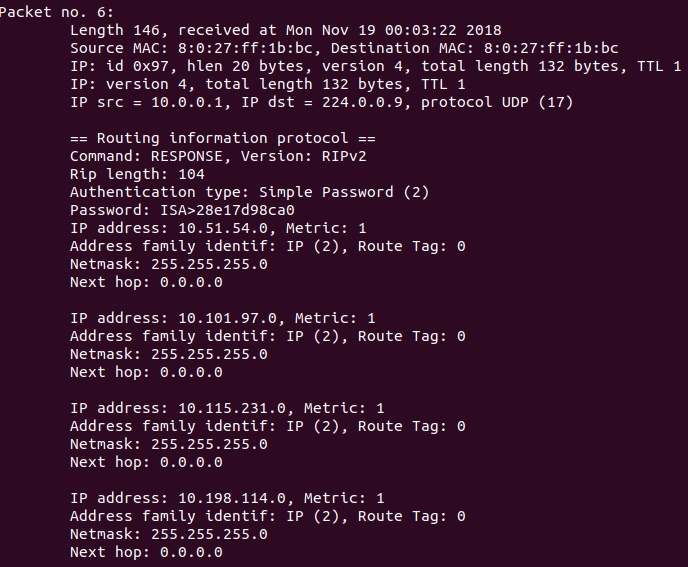
\includegraphics[width=10cm]{img/simple.png} 
	\caption{Sample of captured RIPv2 packet with simple password}
	\label{fig:simple_password}

\end{figure}

\subsubsection{RIPng}
In Figure\ref{fig:ripng} there is an example of captured RIPng packet. It is very similar to RIPv1 and RIPv2 packet described in section \ref{sec:sniffer}. 

\begin{figure}[H]
	
	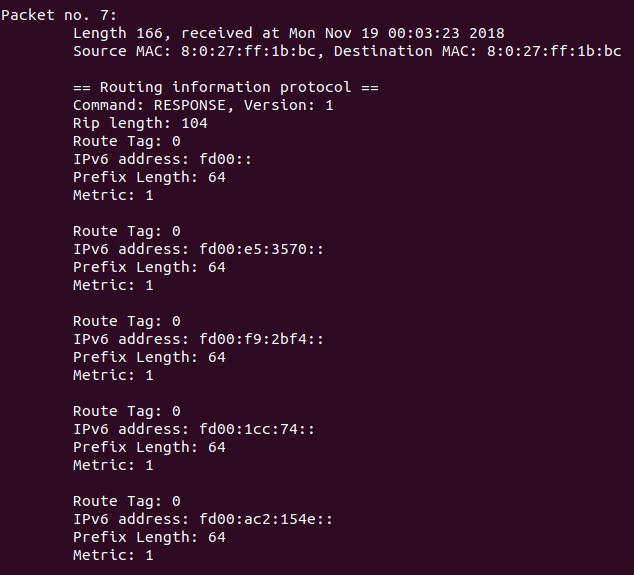
\includegraphics[width=9cm]{img/ipv6.png} 
	\caption{Sample of captured RIPng packet}
	\label{fig:ripng}

\end{figure}

\begin{figure}[H]
	
	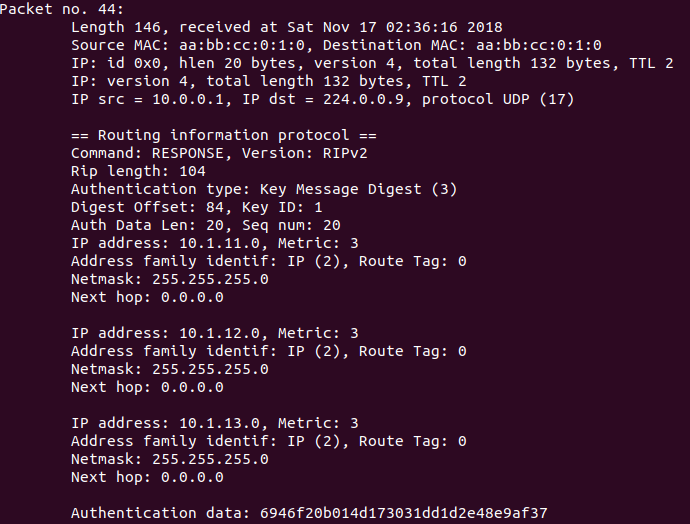
\includegraphics[width=11cm]{img/md5.png} 
	\caption{Sample of captured RIPv2 packet with MD5 password}
	\label{fig:md5}

\end{figure}     

\subsection{Captured routes from FreeBSD}
In tables below there is a list of routes that I captured. The same IP address we can also see in Figure~\ref{fig:simple_password} and Figure~\ref{fig:ripng}.\\

\noindent
\textbf{RIPv2}\\
\begin{tabular}{lccccc}
IPv4 address     & Mask  & NextHop & AFI & Route Tag & Metric\\
\hline
10.51.54.0 		& 255.255.255.0 & 0.0.0.0 & IP & 0 & 1\\
10.101.97.0    & 255.255.255.0 & 0.0.0.0 & IP & 0 & 1\\
10.115.231.0    & 255.255.255.0 & 0.0.0.0 & IP & 0 & 1\\
10.198.114.0    & 255.255.255.0 & 0.0.0.0 & IP & 0 & 1\\
\end{tabular}
\\
\\

\noindent
\textbf{RIPng}\\
\begin{tabular}{lccc}
IPv6 address prefix    & Prefix   & Metric & Route Tag \\
\hline
fd00:: 		& 64  & 1 & 0  \\
fd00:e5:3570:: 		& 64  & 1 & 0  \\
fd00:f9:2bf4::    & 64  & 1 & 0   \\
fd00:1cc:74::    & 64  & 1 & 0   \\
fd00:ac2:154e::    & 64  & 1 & 0   \\
\end{tabular}


\subsection{Sending a fake RIP response packet}
I implemented a program to send RIP response packet with malicious IP address, then by connecting to a router demon ($127.0.0.1 2601$) I could verify that my fake IP address was added to attacked router's routing table (see in Figure~\ref{fig:bsdroute}). In Figure~\ref{fig:send_packet} we can find structure of sent RIPng Response packet visualized in wireshark. \\
\noindent
I got these results by running: \texttt{sudo ./myripresponse -i enp0s3 -r  2001:db8:0:abcd::/64}.

\begin{figure}[H]
	
	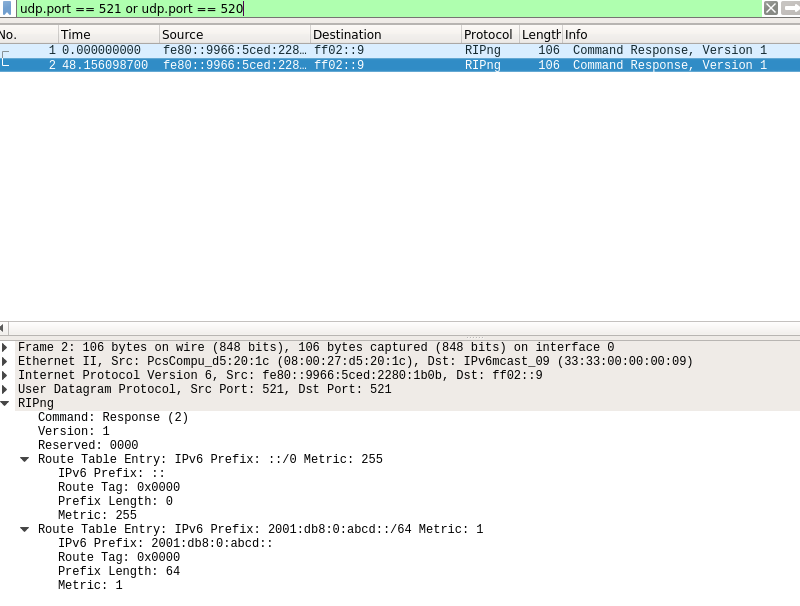
\includegraphics[width=12cm]{img/sendripng.png} 
	\caption{Sample of sent RIPng packet in Wireshark}
	\label{fig:send_packet}

\end{figure}

\begin{figure}[H]
	
	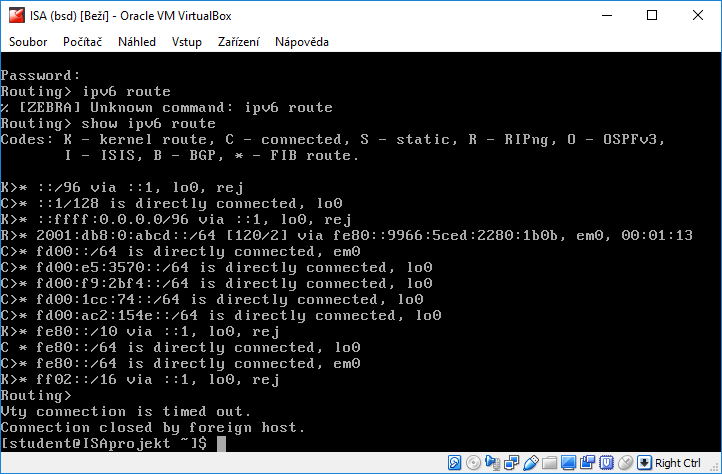
\includegraphics[width=17cm]{img/bsd.png} 
	\caption{Shown routing table on router demon where we can notice a malicious IP address 2001:db8:0:abcd::/64 }
	\label{fig:bsdroute}

\end{figure}

\section{Conclusion}
To summarize, routing information protocols are used to communicate in smaller networks because they have a lot of limitations. RIP prevents routing loops by implementing a limit on the number of hops allowed in a path and uses UDP as a transport protocol on port number 520 and 521. It is based on sending routing table every 30 minutes. The only RIP protocol that contains authentication is RIPv2. As we could see, it is not hard to add fake IP address to a routing table.  

\pagebreak

\begin{thebibliography}{9}
\bibitem{book} 
Jeff Kellum, Mary Ellen Schutz, Patrick J. Conlan, and Christine O'Connor
\textit{Cisco Certified Entry Networking Technician STUDY GUIDE}.  
Neil Edde, Joseph B. Wikert, and Richard Swadley, Indianapolis, Indiana, 2008. ISBN 978-0-470-24702-0.
 
\bibitem{ripv1} 
RFC 1058:  RIP Version 1
\\\url{https://www.ietf.org/rfc/rfc1058.txt}

\bibitem{libpcap} 
Lipcap library
\\\url{http://www.tcpdump.org/}

\bibitem{ripv2} 
RFC 2453:  RIP Version 2
\\\url{https://www.ietf.org/rfc/rfc2453.txt}
 
\bibitem{ripng} 
RFC 2080:  RIPng for IPv6
\\\url{https://www.ietf.org/rfc/rfc2080.txt}

\bibitem{payload} 
RFC 1827: IP Encapsulating Security Payload (ESP)
\\\url{https://www.ietf.org/rfc/rfc1827.txt}

\bibitem{ip_header} 
RFC 1826: IP Authentication Header
\\\url{https://www.ietf.org/rfc/rfc1826.txt}

\bibitem{auth} 
Sample Configuration for Authentication in RIPv2
\\\url{https://www.cisco.com/c/en/us/support/docs/ip/routing-information-protocol-rip/13719-50.html}

\end{thebibliography}

\end{document}
